
\documentclass[12pt, a4paper]{article}

\usepackage{graphicx}
\usepackage{amsmath}
\usepackage{pgfplots}
\pgfplotsset{compat=1.18}
\usepackage{xcolor}
\usepackage{float}
\usepackage{svg}
\usepackage[colorlinks=true, linkcolor=black, urlcolor=blue, citecolor=green]{hyperref}
\usepackage{enumitem}
\usepackage[italian]{babel}
\usepackage{lastpage}  % Pacchetto per ottenere il numero totale delle pagine
\usepackage{fancyhdr}  % Pacchetto per personalizzare l'intestazione e il piè di pagina
\usepackage{tabularx}
\usepackage[margin=1in]{geometry}
\usepackage{array}
\newcolumntype{C}[1]{>{\centering\arraybackslash}p{#1}}
\newcolumntype{L}[1]{>{\raggedright\arraybackslash}p{#1}}
\graphicspath{ {images/} {../shared/images/} }
\definecolor{unipd}{HTML}{B5121B}

\addto\captionsitalian{\renewcommand{\contentsname}{Indice}}

\setcounter{secnumdepth}{5}
\setcounter{tocdepth}{5}
\makeatletter
\newcommand\subsubsubsection{\@startsection{paragraph}{4}{\z@}{-2.5ex\@plus -1ex \@minus -.25ex}{1.25ex \@plus .25ex}{\normalfont\normalsize\bfseries}}
\newcommand\subsubsubsubsection{\@startsection{subparagraph}{5}{\z@}{-2.5ex\@plus -1ex \@minus -.25ex}{1.25ex \@plus .25ex}{\normalfont\normalsize\bfseries}}
\makeatother

\pagestyle{fancy}% Imposta lo stile di pagina su "fancy"
\fancyhf{}% Cancella intestazioni e piè di pagina
\fancyfoot[C]{\thepage{} di \pageref{LastPage}} % Imposta il piè di pagina centrale come "numero pagina di totale pagine"
\renewcommand{\headrulewidth}{0pt} % Imposta la larghezza della linea di intestazione a 0 punti

\newcommand{\data}{}
\newcommand{\titolo}{Piano di qualifica}
%\newcommand{\responsabile}{Responsabile}
\newcommand{\verificatore}{
    & Derek Gusatto \\
    & Alessandro Benin 
}
\newcommand{\redattore}{
    & Matteo Piron \\
    & Matteo Gerardin \\
    & Derek Gusatto
}
\newcommand{\uso}{& Esterno}
\newcommand{\destinatari}{
    & Tullio Vardanega \\
    & Riccardo Cardin \\
    & Vimar S.p.A.
}
\newcommand{\abstractcontent}{ ... }

\begin{document}

\begin{minipage}[]{0.3\textwidth}
\includesvg[width=\linewidth]{pebkac.svg} 
\end{minipage}
\hspace{0.1\textwidth}
\begin{minipage}[]{0.6\textwidth}
  {\Large \textbf{PEBKAC}} \\
  Email: \href{mailto:pebkacswe@gmail.com}{pebkacswe@gmail.com} \\
  Gruppo: 11
\end{minipage}

\bigskip

\begin{minipage}[]{0.3\textwidth}
\includesvg[width=\linewidth]{logo_unipd.svg} 
\end{minipage}
\hspace{0.1\textwidth}
\begin{minipage}[]{0.6\textwidth}
  \textcolor{unipd}{
    \textbf{Università degli Studi di Padova} \\
    Corso di Laurea: Informatica \\
    Corso: Ingegneria del Software \\
    Anno Accademico: 2024/2025
  }
\end{minipage}


\bigskip
\bigskip
\bigskip
\begin{center}
  \Huge\textbf{Verbale Interno}

  \Large\textbf{\data}
\end{center}

\bigskip


\begin{center}
\textbf{Informazioni sul documento}: \\
\vspace{0.5cm}

\begin{tabular}{r|l}
    \textbf{Responsabile} & Tommaso Zocche \\ 
    \textbf{Verificatore} & Alessandro Benin \\ 
    \textbf{Redattore} & Tommaso Zocche \\ 
    \textbf{Uso} & Interno \\ 
    \textbf{Destinatari} & Tullio Vardanega \\ & Riccardo Cardin \\ 
\end{tabular}

\vfill

\textbf{Abstract}: \\
\vspace{0.5cm}
L'obiettivo dell'incontro è stato definire l'ordine di preferenza dei capitolati a seguito degli incontri avuti con le aziende interessate e iniziare a redigere il prospetto orario del gruppo.
\end{center}


\bigskip
\newpage

\section*{Registro delle modifiche}
\begin{table}[H]
    \begin{tabular}{|c|c|c|c|p{5cm}|}
        \hline
         \textbf{Versione} &  \textbf{Data} &  \textbf{Autore} &  \textbf{Ruolo} & \textbf{Descrizione} \\
          \hline
          &  &  & Responsabile & Approvazione e rilascio\\
          \hline
          0.1.0 & 17/11/2024 & Alessandro Benin & Verificatore  & Verificato \\
          \hline
          0.0.1 & 13/11/2024 & Derek Gusatto & Amministratore  & Stesura iniziale \\
          \hline
    \end{tabular}
\end{table}
\newpage
\tableofcontents
\newpage
\listoffigures 
\newpage
\listoftables
\newpage
\section{Introduzione}
\subsection{Scopo del documento}
Il presente documento ha l’obiettivo di definire le \textit{best practices}\textsubscript{G}  e il \textit{way of working}\textsubscript{G} che i componente del team \textit{PEBKAC} hanno l’obbligo di rispettare per l’intero svolgimento del progetto. L'intento è di garantire un metodo di lavoro omogeneo, verificabile
e migliorabile nel tempo. La creazione delle norme è progressiva e incrementale nel tempo per consentire al team di apportare aggiornamenti continui in risposta alle esigenze e alle problematiche incorse durante lo sviluppo dell'intero progetto.

\subsection{Scopo del prodotto}
Il progetto "Vimar GENIALE" mira a sviluppare un'applicazione intelligente che supporti installatori elettrici nell'uso di dispositivi Vimar\textsubscript{G}, facilitando l'accesso alle informazioni tecniche sui prodotti, rispondendo a domande poste in linguaggio naturale.
La tecnologia alla base prevede l'uso di modelli di \textit{LLM}\textsubscript{G} e di tecniche \textit{RAG}\textsubscript{G}, con una struttura di gestione basata su container e integrata in un ambiente cloud.
Il sistema include tre componenti principali: una \textit{applicativo web responsive}\textsubscript{G}, un \textit{applicativo server}\textsubscript{G} e un'\textit{infrastruttura cloud-ready}\textsubscript{G}. 
\subsection{Glossario}
Per evitare ambiguità relative al linguaggio utilizzato nei documenti, viene fornito il Glossario V1.0.0, nel quale si possono trovare tutte le definizioni di termini che hanno un significato specifico che vuole essere disambiguato. Tali termini sono marcati con una G a pedice. 
\subsection{Riferimenti}
\subsubsection{Riferimenti normativi}
\begin{itemize}
    \item Regolamento del progetto didattico\\ \href{https://www.math.unipd.it/~tullio/IS-1/2024/Dispense/PD1.pdf}{https://www.math.unipd.it/~tullio/IS-1/2024/Dispense/PD1.pdf} \\ (Ultimo accesso 2024-11-14)
    \item ISO/IEC 12207:1995 Information technology - Software life cycle processes \\ \href{https://www.math.unipd.it/~tullio/IS-1/2010/Approfondimenti/A03.pdf}{https://www.math.unipd.it/~tullio/IS-1/2010/Approfondimenti/A03.pdf}\\ (Ultimo accesso 2024-11-14)

\end{itemize}

\subsubsection{Riferimenti informativi}
\begin{itemize}
    \item Capitolato C2 \\ \href{https://www.math.unipd.it/~tullio/IS-1/2024/Dispense/PD1.pdf}{https://www.math.unipd.it/~tullio/IS-1/2024/Dispense/PD1.pdf}\\ (Ultimo accesso 2024-11-14)
    \item Capitolato C2 - slides \\ \href{https://www.math.unipd.it/~tullio/IS-1/2024/Dispense/PD1.pdf}{https://www.math.unipd.it/~tullio/IS-1/2024/Dispense/PD1.pdf}\\ (Ultimo accesso 2024-11-14)
    \item Documentazione\textsubscript{G} GitHub\textsubscript{G} \\ \href{https://docs.github.com/en}{https://docs.github.com/en}\\ (Ultimo accesso 2024-11-14)
    
\end{itemize}
\newpage
\section{Qualità di processo}
La qualità di processo si basa sull’idea che, per realizzare un prodotto conforme a specifici standard qualitativi, è essenziale monitorare e migliorare regolarmente i processi che lo generano. Questo principio si applica all’intera gamma di attività, pratiche e metodologie impiegate durante il ciclo di vita del \textit{software\textsubscript{G}}.
In altre parole, la qualità dei processi ha l'obiettivo di andare a conformare la qualità del prodotto in modo tale da garantire sempre che gli standard definidi nel documento \textit{Norme di Progetto} vengano rispettati ed eventualmente migliorati. Di seguito sono elencate le metriche che il team si impegna a rispettare per garantire l’eccellenza nei processi. 
\subsection{Processi primari}
\subsubsection{Fornitura}

\begin{table}[H]
    \centering
    \begin{tabularx}{\textwidth}{>{\hsize=0.5\hsize}X|X|>{\centering\arraybackslash}X|>{\hsize=0.8\hsize}>{\centering\arraybackslash}X}
        \textbf{Metrica} & \textbf{Descrizione} & \textbf{Valore Accettabile} & \textbf{Valore Ideale} \\ \hline
        
         CV& Cost variance& \(\pm\)150 & 0 \\ \hline
         PV& Planned Value& \(\ge 0\) & \(\le BAC\) \\ \hline
         EV& Earned Value& \(\ge 0\) & \(\le EAC\) \\ \hline
         AC& Actual Cost& \(\ge 0\)  & \(\le EAC\) \\ \hline
         CPI& Cost Performance Index & tra 0.95 e 1.05& 1 \\ \hline
         EAC& Estimated At Completion & \(\pm\)5\% del budget preventivato & budget preventivato \\ \hline 
         ETC& Estimated To Completion & \(\ge 0\) & \(\le EAC\) \\ \hline
         SV& Schedule Variance & \(\pm\)150 & 0\% \\ \hline
         BV& Budget Variance & \(\ge\) 10\%  & 0\% \\ \hline
         BAC& Budget At Completion & -  & - \\ 
         
    \end{tabularx}
    \caption{Metriche per il processo di fornitura}
\end{table}

\subsubsection{Sviluppo}
\subsubsubsection{Codifica}

\begin{table}[H]
    \centering
    \begin{tabularx}{\textwidth}{>{\hsize=0.5\hsize}X|X|>{\centering\arraybackslash}X|>{\hsize=0.8\hsize}>{\centering\arraybackslash}X}
   
        \textbf{Metrica} & \textbf{Descrizione} & \textbf{Valore accettabile} & \textbf{Valore ideale}  \\
        \hline
        SC & Statement Coverage &  \(\ge 70\%\) & \(\ge 100\%\) \\
        
    \end{tabularx}
    \caption{Metriche per il processo di codifica}
\end{table}

\subsection{Processi di supporto}

\subsubsection{Documentazione}

\begin{table}[H]
    \centering
    \begin{tabularx}{\textwidth}{>{\hsize=0.5\hsize}X|X|>{\centering\arraybackslash}X|>{\hsize=0.8\hsize}>{\centering\arraybackslash}X}
   
        \textbf{Metrica} & \textbf{Descrizione} & \textbf{Valore accettabile} & \textbf{Valore ideale}  \\
        \hline
        IG & Indice Gulpease & \(\ge65\%\) & 100 \\

        
    \end{tabularx}
    \caption{Metriche per il processo di documentazione}
\end{table}

\subsubsection{Gestione della qualità}

\begin{table}[H]
    \centering
    \begin{tabularx}{\textwidth}{>{\hsize=0.5\hsize}X|X|>{\centering\arraybackslash}X|>{\hsize=0.8\hsize}>{\centering\arraybackslash}X}
   
        \textbf{Metrica} & \textbf{Descrizione} & \textbf{Valore accettabile} & \textbf{Valore ideale}  \\
        \hline
        MNS & Metriche Non Soddisfatte & \(\le3\) & 0\\
        
    \end{tabularx}
    \caption{Metriche per il processo di gestione delle qualità}
\end{table}


\newpage
\section{Qualità del prodotto}
La qualità del prodotto si concentra sulla valutazione del \textit{software}\textsubscript{G} sviluppato, ponendo l'accento su caratteristiche come facilità d'uso, funzionalità\textsubscript{G}, affidabilità\textsubscript{G}, capacità di manutenzione\textsubscript{G} e, in senso più ampio, sulle prestazioni complessive del prodotto. L'obiettivo principale del \textit{team}\textsubscript{G} è anche quello non solo di soddisfare le attese del cliente fornendo un prodotto \textit{software}\textsubscript{G} che implementi le funzionalità\textsubscript{G} volute, ma che lo faccia seguendo precisi \textit{standard}\textsubscript{G} di qualità. Vengono quindi fornite di seguito le metriche\textsubscript{G} che il \textit{team}\textsubscript{G} si impegna a soddisfare nel contesto della qualità del prodotto. 

\subsection{Funzionalità}

\begin{table}[H]
    \centering
    \begin{tabularx}{\textwidth}{>{\hsize=0.5\hsize}X|X|>{\centering\arraybackslash}X|>{\hsize=0.8\hsize}>{\centering\arraybackslash}X}
   
        \textbf{Metrica} & \textbf{Descrizione} & \textbf{Valore accettabile} & \textbf{Valore ideale}  \\
        \hline
        ROS\textsubscript{G} & Requisiti Obbligatori Soddisfatti & \(100\%\) & 0\\
        \hline
        RDS\textsubscript{G} & Requisiti Desiderabili Soddisfatti & \(\ge0\%\) & \(\ge75\%\)\\
        \hline
        RPS\textsubscript{G} & Requisiti Opzionali Soddisfatti & \(\ge0\%\) & \(\ge50\%\)\\
        
    \end{tabularx}
    \caption{Metriche\textsubscript{G} per la funzionalità\textsubscript{G} del prodotto}
\end{table}

\subsection{Manutenibilità}

\begin{table}[H]
    \centering
    \begin{tabularx}{\textwidth}{>{\hsize=0.5\hsize}X|X|>{\centering\arraybackslash}X|>{\hsize=0.8\hsize}>{\centering\arraybackslash}X}
   
        \textbf{Metrica} & \textbf{Descrizione} & \textbf{Valore accettabile} & \textbf{Valore ideale}  \\
        \hline
        SFIN\textsubscript{G} & \textit{Structure Fan In}\textsubscript{G} & da determinare & da determinare\\
        \hline
        SFOUT\textsubscript{G} & \textit{Structure Fan Out}\textsubscript{G} & da determinare & da determinare\\
        
    \end{tabularx}
    \caption{Metriche\textsubscript{G} per la manutenibilità\textsubscript{G} del prodotto}
\end{table}

\subsection{Affidabilità}

\begin{table}[H]
    \centering
    \begin{tabularx}{\textwidth}{>{\hsize=0.5\hsize}X|X|>{\centering\arraybackslash}X|>{\hsize=0.8\hsize}>{\centering\arraybackslash}X}
   
        \textbf{Metrica} & \textbf{Descrizione} & \textbf{Valore accettabile} & \textbf{Valore ideale}  \\
        \hline
        PTCP\textsubscript{G} & \textit{Passed Test Cases Percentage}\textsubscript{G} & \(\ge80\%\) & \(100\%\)\\
        \hline
        CC\textsubscript{G} & \textit{Code Coverage}\textsubscript{G} & \(\ge80\%\) & \(100\%\)\\
        
    \end{tabularx}
    \caption{Metriche\textsubscript{G} per l'affidabilità\textsubscript{G} del prodotto}
\end{table}

\subsection{Efficienza}

\begin{table}[H]
    \centering
    \begin{tabularx}{\textwidth}{>{\hsize=0.5\hsize}X|X|>{\centering\arraybackslash}X|>{\hsize=0.8\hsize}>{\centering\arraybackslash}X}
   
        \textbf{Metrica} & \textbf{Descrizione} & \textbf{Valore accettabile} & \textbf{Valore ideale}  \\
        \hline
        TDE\textsubscript{G} & Tempo Di Elaborazione\textsubscript{G} & da determinare & da determinare\\
        
    \end{tabularx}
    \caption{Metriche\textsubscript{G} per l'efficienza del prodotto}
\end{table}

\newpage
\section{Strategie di testing}
Per dimostare che i requisiti individuati dagli analisti ed elencati nella sezione omonima dell'Analisi dei Requisiti siano soddisfatti, è necessario che vengano realizzati dei test appositi che verranno eseguiti sul prodotto sia in fase di codifica che in fase di verifica e revisione.\\
I test realizzabili possono essere suddivisi in quattro categorie principali:
\begin{itemize}
    \item \textbf{Test di unità}: verificano il corretto funzionamento di una singola unità di codice indipendente (ad esempio una funzione), assicurandosi che produca i risultati attesi al variare dei possibili input\textsubscript{G}, e vengono generalmente automatizzati per facilitare l'individuazione degli errori durante la fase di sviluppo;
    \item \textbf{Test di integrazione}: verificano il corretto funzionamento delle interazioni tra diverse unità di codice o componenti di un sistema, assicurandosi che, una volta integrati, i vari moduli lavorino insieme senza problemi, rilevando eventuali errori nelle interfacce e nei flussi di dati tra di essi;
    \item \textbf{Test di sistema}: verificano il comportamento complessivo di un'intera applicazione o sistema, testando tutte le sue componenti integrate per assicurarsi che soddisfi i requisiti funzionali e non funzionali, assicurandosi di valutare il sistema nel suo insieme simulando l'uso reale per identificare eventuali problemi di performance, sicurezza o compatibilità;
%    \item \textbf{Test End-to-End}: verificano il funzionamento complessivo di un sistema eseguendo casi d'uso dall'inizio alla fine, comprese le interazioni con altri sistemi o applicazioni esterne, per garantire il corretto funzionamento di tutti gli elementi insieme, simulando l'esperienza dell'utente in un contesto realistico.
    \item \textbf{Test di accettazione}: verificano se un sistema o una parte di esso soddisfa i requisiti e le aspettative degli utenti o del cliente, venendo eseguiti prima del rilascio del software per confermare che il prodotto finale sia pronto per l'uso e conforme alle specifiche concordate.
\end{itemize}

\subsection{Notazione dei test}
\'E stato decisa come notazione per identificare univocamente i test la seguente:
\begin{center}
    \textbf{T[Tipologia][Numero]}
\end{center}
\textbf{Tipologia} indica la tipologia del test:
\begin{itemize}
    \item \textbf{U}: di unità;
    \item \textbf{I}: di integrazione;
    \item \textbf{S}: di sistema;
%    \item \textbf{E}: End-to-End;
    \item \textbf{A}: di accettazione.
\end{itemize}
Ogni test si trova in uno \textbf{Stato}, che può essere:
\begin{itemize}
    \item \textbf{V}: verificato. Questo stato indica che il test ha fornito un esito positivo;
    \item \textbf{NV}: non verificato. Questo stato indica che il test ha fornito un esito negativo;
    \item \textbf{NI}: non implementato. Questo stato indica che il test non è ancora stato implementato, e quindi non fornisce nessun esito.
\end{itemize}

\subsection{Test di unità}
I test di unità sono una tipologia di test utilizzata per verificare singoli componenti o unità di codice in isolamento, al fine di garantire che funzionino correttamente. Un'unità di codice può essere una funzione, un metodo, una classe o un modulo, a seconda del livello di granularità scelto. I test di unità vengono solitamente scritti dagli sviluppatori durante o immediatamente dopo la scrittura del codice e vengono utilizzati per:
\begin{itemize}
    \item Validare il comportamento del codice, assicurandosi che ogni unità fornisca risultati corretti per un determinato insieme di input;
    \item Facilitare la manutenzione del software, individuando rapidamente errori introdotti da modifiche;
    \item Promuovere la modularità, progettando concettualmente componenti indipendenti e riutilizzabili.
\end{itemize}
Per la realizzazione di questa categoria di \textit{test\textsubscript{G}} per questo progetto saranno utilizzati i \textit{framework Pytest\textsubscript{G}} e \textit{unittest\textsubscript{G}} per Python, dato che quest'ultimo è il linguaggio scelto per la realizzazione del \textit{backend\textsubscript{G}}.\\
I test di unità, insieme ai test di integrazione, come richiesto nel capitolato, devono avere un coverage minimo pari al 75\% (opzionalmente un coverage minimo pari al 90\%).
%TODO: Inserire i test
%\begin{table}[H]
%    \centering
%    \begin{tabularx}{\textwidth}{>{\hsize=0.2\hsize}>{\centering\arraybackslash}X|X|>{\hsize=0.1\hsize}>{\centering\arraybackslash}X}
%        \textbf{Codice} & \textbf{Descrizione} & \textbf{Stato} \\
%        \hline
%        TU-1 &  & NI \\
%        \hline
%        TU-2 &  & NI \\
%        \hline
%        TU-3 &  & NI \\
%    \end{tabularx}
%    \caption{Stato dei test di unità}
%\end{table}

\subsection{Test di integrazione}
I test di integrazione sono una tipologia di test progettata per verificare la capacità di diversi componenti o moduli di un sistema di funzionare insieme. I test di integrazione non mirano a testare singoli moduli in modo indipendente, come fa il test di unità, che si concentra su unità di codice isolate. Le caratteristiche principali dei test di integrazione sono:
\begin{itemize}
    \item Monitorare i problemi di comunicazione tra moduli;
    \item Garantire la corretta configurazione e gestione delle dipendenze tra moduli;
    Testare il sistema in condizioni più vicine a quelle reali rispetto a quanto avviene con i test di unità.
\end{itemize}
I test di integrazione, insieme ai test di unità, come richiesto nel capitolato, devono avere un coverage minimo pari al 75\% (opzionalmente un coverage minimo pari al 90\%).
%TODO: Inserire i test
%\begin{table}[H]
%    \centering
%    \begin{tabularx}{\textwidth}{>{\hsize=0.2\hsize}>{\centering\arraybackslash}X|X|>{\hsize=0.1\hsize}>{\centering\arraybackslash}X}
%        \textbf{Codice} & \textbf{Descrizione} & \textbf{Stato} \\
%        \hline
%        TI-1 &  & NI \\
%        \hline
%        TI-2 &  & NI \\
%        \hline
%        TI-3 &  & NI \\
%    \end{tabularx}
%    \caption{Stato dei test di unità}
%\end{table}

\subsection{Test di sistema}
I test di sistema sono una tipologia di test attraverso la quale vengono testati il comportamento e la funzionalità di un sistema completo nel suo insieme. Viene eseguito dopo che tutti i componenti o moduli sono stati integrati e serve a garantire che il sistema soddisfi i requisiti funzionali e non funzionali specificati. I test di sistema valutano il software in un ambiente il più possibile vicino a quello reale, simulando gli utenti di tale software. Le caratteristiche chiave dei test di sistema sono:
\begin{itemize}
    \item Verifica dei requisiti funzionali: assicurarsi che il sistema fornisca le funzionalità previste;
    \item Verifica dei requisiti non funzionali: verifica di prestazioni, sicurezza, usabilità, scalabilità...
    \item Test End-to-End: valutazione di flussi di lavoro completi, inclusa l'interazione con altri sistemi o applicazioni esterne;
    \item Valutazione della conformità: garantire che il sistema aderisca a specifici standard o regolamenti.
\end{itemize}
%TODO: Inserire i test
\begin{table}[H]
    \centering
    \begin{tabularx}{\textwidth}{>{\hsize=0.3\hsize}>{\centering\arraybackslash}X|X|>{\hsize=0.4\hsize}>{\centering\arraybackslash}X|>{\hsize=0.2\hsize}>{\centering\arraybackslash}X}
        \textbf{Codice} & \textbf{Descrizione} & \textbf{Requisito} & \textbf{Stato} \\
        \hline
TS-1 & Il sistema deve permettere al modulo AI di interrogare il database in modo efficace per recuperare informazioni sui prodotti. Le informazioni restituite devono essere corrette, coerenti e aggiornate, garantendo che gli utenti ottengano risposte utili per le loro domande. & RF.O.026, RF.O.027 & NI \\
\hline
TS-2 & Deve essere garantita l'integrazione fluida tra il frontend e il backend, con l'elaborazione delle richieste degli utenti tramite GUI\textsubscript{G} e la restituzione di risposte tempestive e accurate nella stessa interfaccia. & UC1, UC6 & NI \\
\hline
TS-3 & Quando l'utente inserisce una domanda che supera il limite di caratteri predefinito, il sistema deve gestire questa situazione restituendo un messaggio di errore chiaro e comprensibile. & RF.O.009, UC7 & NI \\
\hline
TS-4 & La pipeline\textsubscript{G} di estrazione automatizzata dei dati dal sito Vimar deve raccogliere e indicizzare in modo efficiente le informazioni, rendendole disponibili per le interrogazioni degli utenti. & RF.O.020, RF.O.025 & NI \\
\hline
TS-5 & Il sistema deve essere avviabile tramite Docker Compose\textsubscript{G} e garantire che tutti i componenti dell'infrastruttura containerizzata funzionino correttamente in un ambiente scalabile e portabile. & RV.O.002, RV.O.007 & NI \\
\hline
TS-6 & La dashboard\textsubscript{G} amministrativa deve fornire agli amministratori una panoramica chiara e aggiornata sull'utilizzo del sistema, incluse statistiche dettagliate sulle richieste effettuate dagli utenti. & RF.O.003, UC14 & NI \\
\hline
TS-7 & La pipeline di indicizzazione automatizzata deve operare senza interventi manuali, consentendo l'aggiornamento continuo delle informazioni nel database in base ai nuovi dati raccolti. & RF.O.025, RF.O.026 & NI \\
\hline
TS-8 & Deve essere possibile estrarre correttamente informazioni utili dai file PDF, inclusi schemi elettrici e manuali tecnici, rendendoli disponibili per la consultazione e il download. & RF.O.023, RF.D.022 & NI \\
\hline
TS-9 & Il sistema deve identificare e gestire richieste relative a argomenti proibiti, restituendo un messaggio appropriato che informa l'utente della restrizione. & RF.O.005, UC15 & NI \\
\hline
\end{tabularx}
 \end{table}
 \begin{table}[H]
    \centering
    \begin{tabularx}{\textwidth}{>{\hsize=0.3\hsize}>{\centering\arraybackslash}X|X|>{\hsize=0.4\hsize}>{\centering\arraybackslash}X|>{\hsize=0.2\hsize}>{\centering\arraybackslash}X}
        \textbf{Codice} & \textbf{Descrizione} & \textbf{Requisito} & \textbf{Stato} \\
        \hline
TS-10 & L'infrastruttura del sistema deve supportare la scalabilità, consentendo l'esecuzione simultanea su più nodi senza compromettere le prestazioni o l'affidabilità. & RQ.O.002, RV.O.007 & NI \\
\hline
TS-11 & Il sistema deve funzionare correttamente su tutti i browser compatibili specificati, garantendo un'esperienza utente coerente e priva di errori. & RV.O.012 - RV.O.016 & NI \\
\hline
TS-12 & Le \textit{API\textsubscript{G}} devono essere protette con meccanismi di autenticazione adeguati, come le API-Key, per garantire accessi sicuri e controllati ai servizi del sistema. & RV.O.006, RF.O.027 & NI \\
\hline
TS-13 & Il database deve essere aggiornabile con nuove informazioni sui prodotti in modo che il sistema possa fornire risposte aggiornate e precise agli utenti. & RF.O.021, RF.O.024 & NI \\
\hline
TS-14 & La dashboard deve mostrare statistiche aggiornate in tempo reale, consentendo agli amministratori di monitorare l'utilizzo del sistema con una visione dinamica e dettagliata. & RF.P.016, UC14.3 & NI \\
\hline
TS-15 & Il sistema deve supportare sessioni multiple di utenti simultanei, garantendo l'isolamento delle sessioni e l'integrità dei dati per ciascun utente. & RQ.D.001, UC1 & NI \\
\hline
TS-16 & Il sistema deve essere in grado di rispondere accuratamente a domande poste in lingua italiana, utilizzando il modello AI per generare risposte appropriate. & RF.O.001, UC16 & NI \\
\hline
TS-17 & Le sessioni di conversazione devono poter essere salvate e recuperate senza perdita di dati, consentendo agli utenti di riprendere le interazioni da dove erano state interrotte. & RF.O.012, UC3 & NI \\
\hline
TS-18 & Le risposte del sistema devono includere immagini o schemi tecnici, quando richiesto, garantendo la loro corretta visualizzazione nell'interfaccia utente. & RF.O.027, UC17 & NI \\
\hline
TS-19 & La dashboard amministrativa deve fornire statistiche dettagliate sui feedback ricevuti dagli utenti, inclusi conteggi di risposte positive e negative. & RF.D.019, UC14.5 & NI \\
\hline
TS-20 & Gli utenti devono poter ricercare e recuperare conversazioni salvate in precedenza, garantendo l'accesso a tutte le informazioni contenute nelle conversazioni archiviate. & RF.P.040, UC9 & NI \\
\hline
\end{tabularx}
 \end{table}
 \begin{table}[H]
    \centering
    \begin{tabularx}{\textwidth}{>{\hsize=0.3\hsize}>{\centering\arraybackslash}X|X|>{\hsize=0.4\hsize}>{\centering\arraybackslash}X|>{\hsize=0.2\hsize}>{\centering\arraybackslash}X}
        \textbf{Codice} & \textbf{Descrizione} & \textbf{Requisito} & \textbf{Stato} \\
\hline
TS-21 & Il sistema deve gestire la situazione in maniera corretta e mostrare un messaggio di errore chiaro e dettagliato nel caso in cui un utente tenti di salvare una conversazione senza che ne sia stata creata alcuna. & UC4, RF.O.034 & NI \\
\hline
TS-22 & Il sistema deve consentire all'installatore di visualizzare la data e l'ora di invio di ogni messaggio nella cronologia delle conversazioni. & RF.P.041, RF.P.042 & NI \\
\hline
TS-23 & Il sistema deve consentire agli amministratori di azzerare il conteggio dei \textit{feedback\textsubscript{G}} positivi e negativi ricevuti, mostrando un messaggio di conferma. & RF.P.044, RF.P.045 & NI \\
\hline
TS-24 & Il sistema supporta correttamente la creazione di nuove sessioni di conversazione, garantendo che siano archiviate e accessibili successivamente. & RF.O.035, UC1 & NI \\
\hline
TS-25 & Il sistema consente agli utenti di accedere al contenuto dei documenti di interesse direttamente dalla risposta fornita. & RF.P.043, UC17 & NI \\
\hline
TS-26 & L'interfaccia utente del sistema deve essere completamente responsive, adattandosi a diversi dispositivi senza errori di layout. & RQ.D.001 & NI \\
\hline
TS-27 & Il sistema deve inviare un avviso in caso di errore durante l'indicizzazione automatica dei dati provenienti dal sito Vimar. & RF.O.025, RF.O.026 & NI \\
\hline
TS-28 & Il sistema deve includere una funzione di "ripristino" per le sessioni interrotte a causa di errori tecnici, garantendo che nessun dato venga perso. & UC3, RF.O.012 & NI \\
\hline
TS-29 & Il sistema deve mostrare un messaggio chiaro quando l'utente cerca di accedere alla dashboard con credenziali errate. & UC13 & NI \\
\hline
TS-30 & Il sistema deve restituire un messaggio specifico quando non esistono messaggi pregressi nella cronologia della conversazione selezionata. & UC10 & NI \\
\hline
TS-31 & Il sistema deve restituire un messaggio chiaro e dettagliato quando si tenta di accedere a una funzionalità riservata agli amministratori senza aver effettuato l'accesso. & UC12 & NI \\
\hline
TS-32 & Il sistema deve garantire che, durante la ricerca di informazioni, vengano restituiti solo prodotti pertinenti alla categoria selezionata dall’installatore. & UC6 & NI \\
    \end{tabularx}
    \caption{Stato dei test di sistema}
\end{table}

%\subsection{Test End-to-End}
%I test End-to-End sono una tipologia di test che valida il funzionamento complessivo di un sistema, testando l'intero flusso dal punto A al punto B. Questo tipo di test riguarda l'interazione tra le parti del sistema stesso e con sistemi esterni, per assicurarsi che tutte le parti funzionino correttamente insieme, emulando una situazione online da testare tramite l'utente finale. In questo modo, si garantisce che il sistema sia privo di errori, soddisfi i requisiti funzionali e contribuisca a una buona esperienza utente.
%I test End-to-End, come richiesto nel capitolato, devono avere un coverage minimo pari all'80\%.
%TODO: Inserire i test
%\begin{table}[H]
%    \centering
%    \begin{tabularx}{\textwidth}{>{\hsize=0.4\hsize}>{\centering\arraybackslash}X|X|>{\centering\arraybackslash}X|>{\hsize=0.3\hsize}>{\centering\arraybackslash}X}
%        \textbf{Codice} & \textbf{Descrizione} & \textbf{Casi d'uso} & \textbf{Stato} \\
%        \hline
%        TE-1 &  &  & NI \\
%        \hline
%        TE-2 &  &  & NI \\
%        \hline
%        TE-3 &  &  & NI \\
%    \end{tabularx}
%    \caption{Stato dei test End-to-End}
%\end{table}

\subsection{Test di accettazione}
I test di accettazione sono una tipologia di test che verifica che un sistema o un'applicazione soddisfi requisiti ed aspettative concordate con il cliente o contro l'utente finale. Normalmente, questi test sono condotti sul ciclo finale del processo di sviluppo, prima della pubblicazione o della consegna del prodotto. Questi test hanno l'obiettivo di:
\begin{itemize}
    \item Confermare la conformità ai requisiti funzionali: verificare che il sistema realizzi le funzionalità richieste;
    \item Verificare che sia appropriato per l'utilizzo nel mondo reale: assicurarsi che il sistema sia pronto per un ambiente di produzione.
    \item Dare all'ente proprietario la capacità di approvare o rifiutare il sistema: un test di accettazione di successo è proprio l'ultimo passo di approvazione per il rilascio.
\end{itemize}
%TODO: Inserire i test
\begin{table}[H]
    \centering
    \begin{tabularx}{\textwidth}{>{\hsize=0.4\hsize}>{\centering\arraybackslash}X|X|>{\centering\arraybackslash}X|>{\hsize=0.3\hsize}>{\centering\arraybackslash}X}
        \textbf{Codice} & \textbf{Descrizione} & \textbf{Casi d'uso} & \textbf{Stato} \\
        \hline
        TA-1 & Il sistema deve consentire a un installatore di inserire una richiesta tramite conversazione libera e ricevere informazioni dettagliate, incluse descrizioni dei prodotti, schemi elettrici e manuali tecnici. & UC6 & NI \\
\hline

       TA-2 & Un amministratore deve poter accedere alla dashboard inserendo credenziali corrette, garantendo l'accesso solo a utenti autorizzati. & UC12 & NI \\
\hline
TA-3 & Gli utenti devono poter fornire feedback sull'accuratezza delle risposte ricevute, e il sistema deve registrare correttamente tali feedback. & UC11 & NI \\  
\hline
TA-4 & Il sistema deve consentire agli utenti di salvare le conversazioni e confermare che il salvataggio sia avvenuto con successo. & UC3 & NI \\
\hline
TA-5 & Le richieste relative a argomenti non pertinenti devono essere bloccate, e il sistema deve restituire un messaggio di cortesia senza fornire ulteriori risposte. & UC15 & NI \\
\hline
TA-6 & Gli utenti devono poter visualizzare lo storico delle conversazioni in corso, con tutte le risposte mostrate in ordine cronologico. & UC9 & NI \\
\hline
TA-7 & Deve essere possibile eliminare una conversazione salvata, con conferma visibile dell'avvenuta cancellazione. & UC5 & NI \\
\hline
TA-8 & Nel caso in cui venga superato il limite massimo di conversazioni consentite, il sistema deve notificare l'utente con un messaggio chiaro. & UC2 & NI \\
\hline
\end{tabularx}
\end{table}
\begin{table}[H]
    \centering
    \begin{tabularx}{\textwidth}{>{\hsize=0.4\hsize}>{\centering\arraybackslash}X|X|>{\centering\arraybackslash}X|>{\hsize=0.3\hsize}>{\centering\arraybackslash}X}
        \textbf{Codice} & \textbf{Descrizione} & \textbf{Casi d'uso} & \textbf{Stato} \\
        \hline
TA-9 & Gli amministratori devono poter accedere a statistiche di utilizzo tramite la dashboard, con informazioni dettagliate su tutte le richieste effettuate. & UC14 & NI \\
\hline
TA-10 & Gli amministratori devono poter visualizzare il numero di richieste effettuate tramite conversazione libera, direttamente dalla dashboard. & UC14.1 & NI \\
\hline
TA-11 & Gli utenti devono confermare l'eliminazione delle conversazioni salvate prima che queste vengano definitivamente rimosse dal sistema. & UC5 & NI \\
\hline
TA-12 & Il sistema deve fornire risposte dettagliate e accurate relative a prodotti appartenenti agli impianti Smart, su richiesta dell'utente. & UC6 & NI \\
\hline
TA-13 & Gli utenti devono ricevere risposte chiare e precise per prodotti relativi agli impianti Domotici, con tutte le informazioni pertinenti. & UC6 & NI \\
\hline
TA-14 & Il sistema deve estrarre automaticamente informazioni dal sito di Vimar e indicizzarle correttamente per consentire interrogazioni rapide. & UC6 & NI \\
\hline
TA-15 & Deve essere garantita la gestione di richieste per prodotti non presenti, con un messaggio di cortesia che informa l'utente dell'assenza di dati. & UC8 & NI \\
\hline
TA-16 & Gli utenti devono poter scaricare documenti PDF, come manuali tecnici, direttamente dal sistema. & UC17 & NI \\
\hline
TA-17 & Nel caso di superamento del limite massimo di caratteri consentiti in una domanda, il sistema deve notificare l'errore in modo chiaro. & UC7 & NI \\
\hline
\end{tabularx}
\end{table}
\begin{table}[H]
    \centering
    \begin{tabularx}{\textwidth}{>{\hsize=0.4\hsize}>{\centering\arraybackslash}X|X|>{\centering\arraybackslash}X|>{\hsize=0.3\hsize}>{\centering\arraybackslash}X}
        \textbf{Codice} & \textbf{Descrizione} & \textbf{Casi d'uso} & \textbf{Stato} \\
        \hline
TA-18 & Utilizzando un menù guidato, gli utenti devono poter accedere facilmente alle informazioni sui prodotti di loro interesse. & UC18 & NI \\
\hline
TA-19 & Il sistema deve restituire risposte che includano immagini, come schemi elettrici, garantendo la loro corretta visualizzazione nell'interfaccia utente. & UC17 & NI \\
\hline
TA-20 & Gli amministratori devono avere accesso a statistiche relative ai feedback positivi ricevuti, visualizzandole nella dashboard in modo dettagliato. & UC14.4 & NI \\
\hline
TA-21 & Gli installatori devono ricevere un messaggio di conferma visibile quando forniscono feedback sul sistema. & UC11 & NI \\
\hline
TA-22 & Gli installatori devono poter recuperare una lista delle loro conversazioni salvate, con possibilità di visualizzare il contenuto completo di ciascuna. & UC9 & NI \\
\hline
TA-23 & Gli amministratori devono poter visualizzare il numero di richieste effettuate tramite conversazione libera, direttamente dalla dashboard. & UC14.2 & NI \\
\hline
TA-24 & Gli utenti devono poter interrompere una conversazione guidata e tornare al menu principale senza perdere lo storico delle interazioni effettuate fino a quel momento. & UC5 & NI \\
\hline
TA-25 & Gli amministratori devono poter visualizzare le statistiche aggiornate sul numero di parole utilizzate nelle richieste, direttamente dalla dashboard. & UC14.3 & NI \\
    \end{tabularx}
    \caption{Stato dei test di accettazione}
\end{table}
\newpage
\section{Cruscotto delle metriche}
\subsection{Qualità di processo - Fornitura}
\subsubsection{Earned Value, Actual Cost, Planned Value}
\begin{figure}[H]
    \centering
    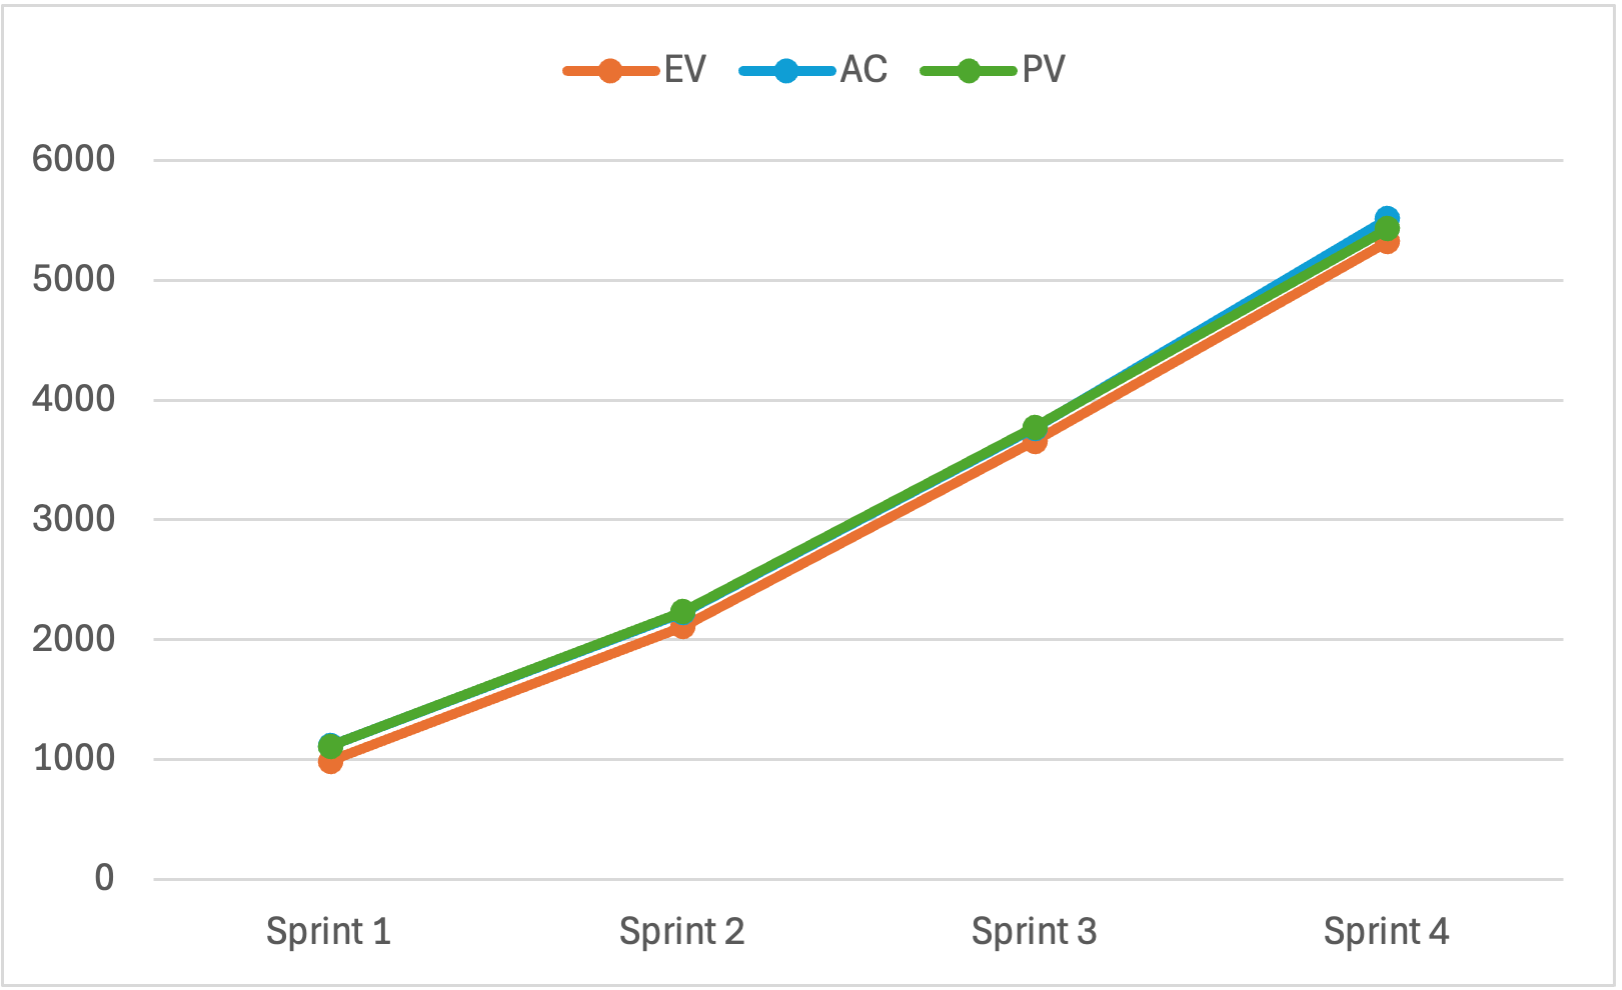
\includegraphics[width=0.8\textwidth]{./images/EV-AC-PV.png}
    \caption{Earned Value, Actual Cost, Planned Value}
\end{figure}
\subsubsubsection*{Analisi}
Queste metriche indicano un buon andamento essenso sempre abbastanza sovrapposte su tutti gli sprint, anche se si nota in graduale distaccamento verso il quarto sprint a causa dell'aumento dei costi per il raggiungimento degli obiettivi.

\subsubsection{Estimated To Compliation, Estimated At Compliation}
\begin{figure}[H]
    \centering
    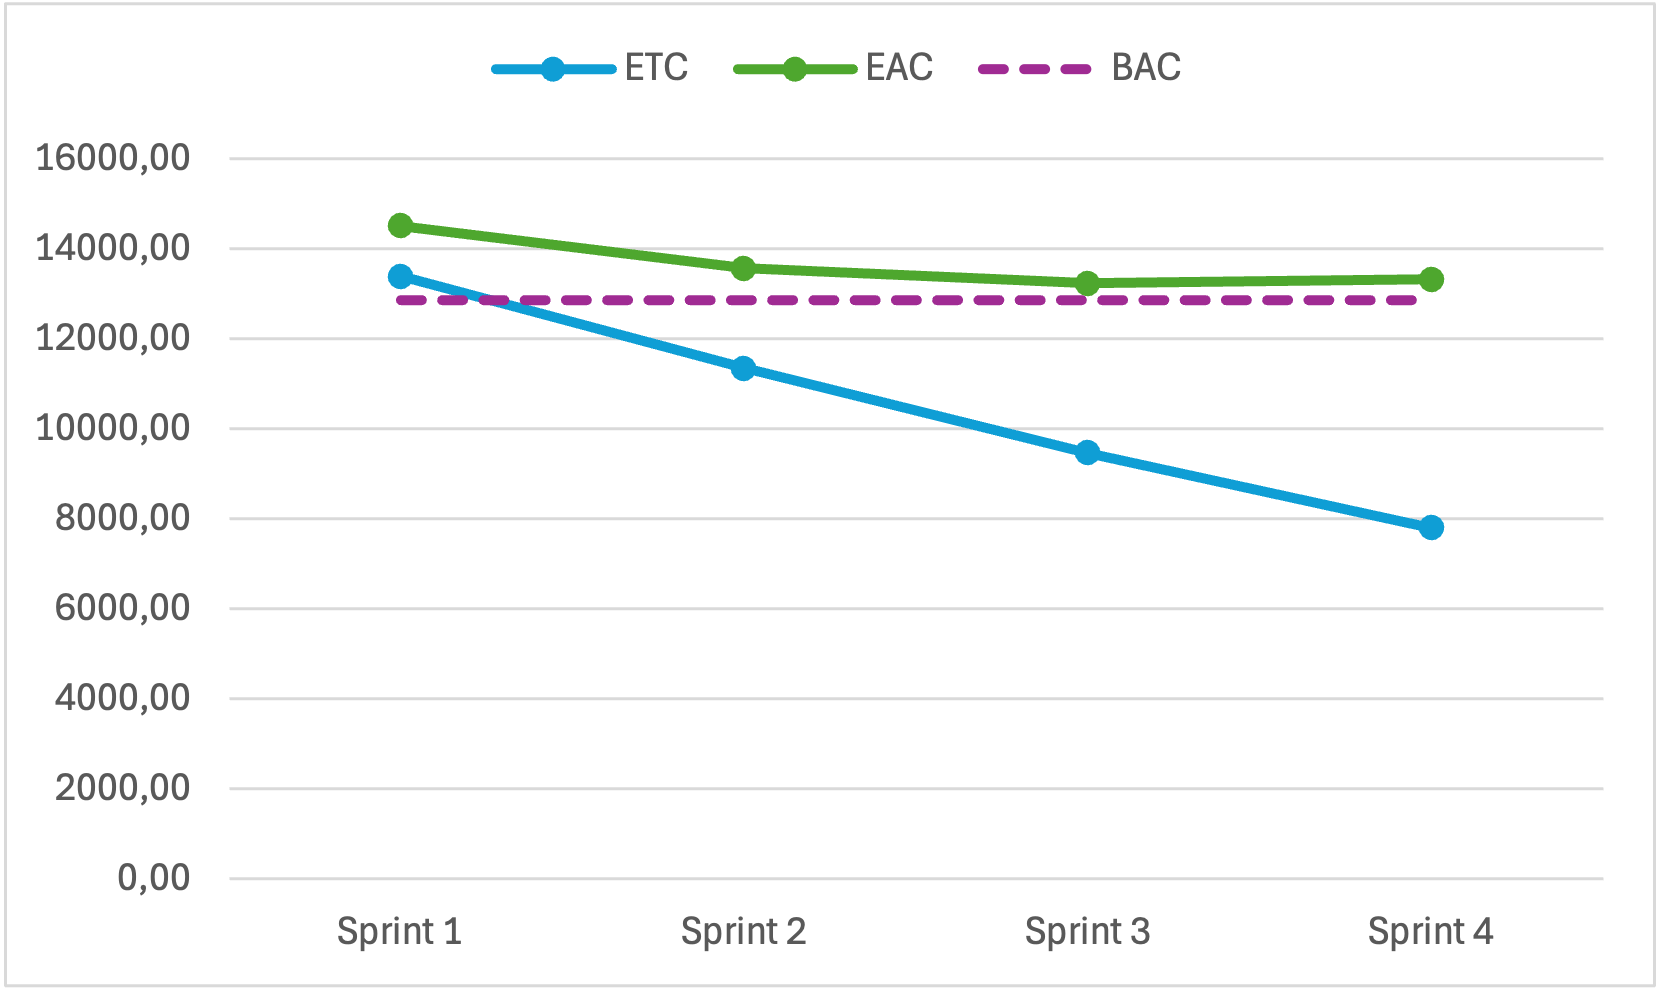
\includegraphics[width=0.8\textwidth]{./images/ETC-EAC.png}
    \caption{Estimated To Compliation, Estimated At Compliation}
\end{figure}
\subsubsubsection*{Analisi}
Dopo un inizio non ottimale è possibile notare un riallineamento. L'Estimation At Completion si è riallineato al Badget At Completion, ma è sempre rimasto superiore, anche se di poco, a causa del costo maggiore per il raggiungimento di tutti gli obiettivi degli sprint. L'Estimated To Commpletion è sempre stato gradualmente discendente.
\subsubsection{Budget Variance}
\begin{figure}[H]
    \centering
    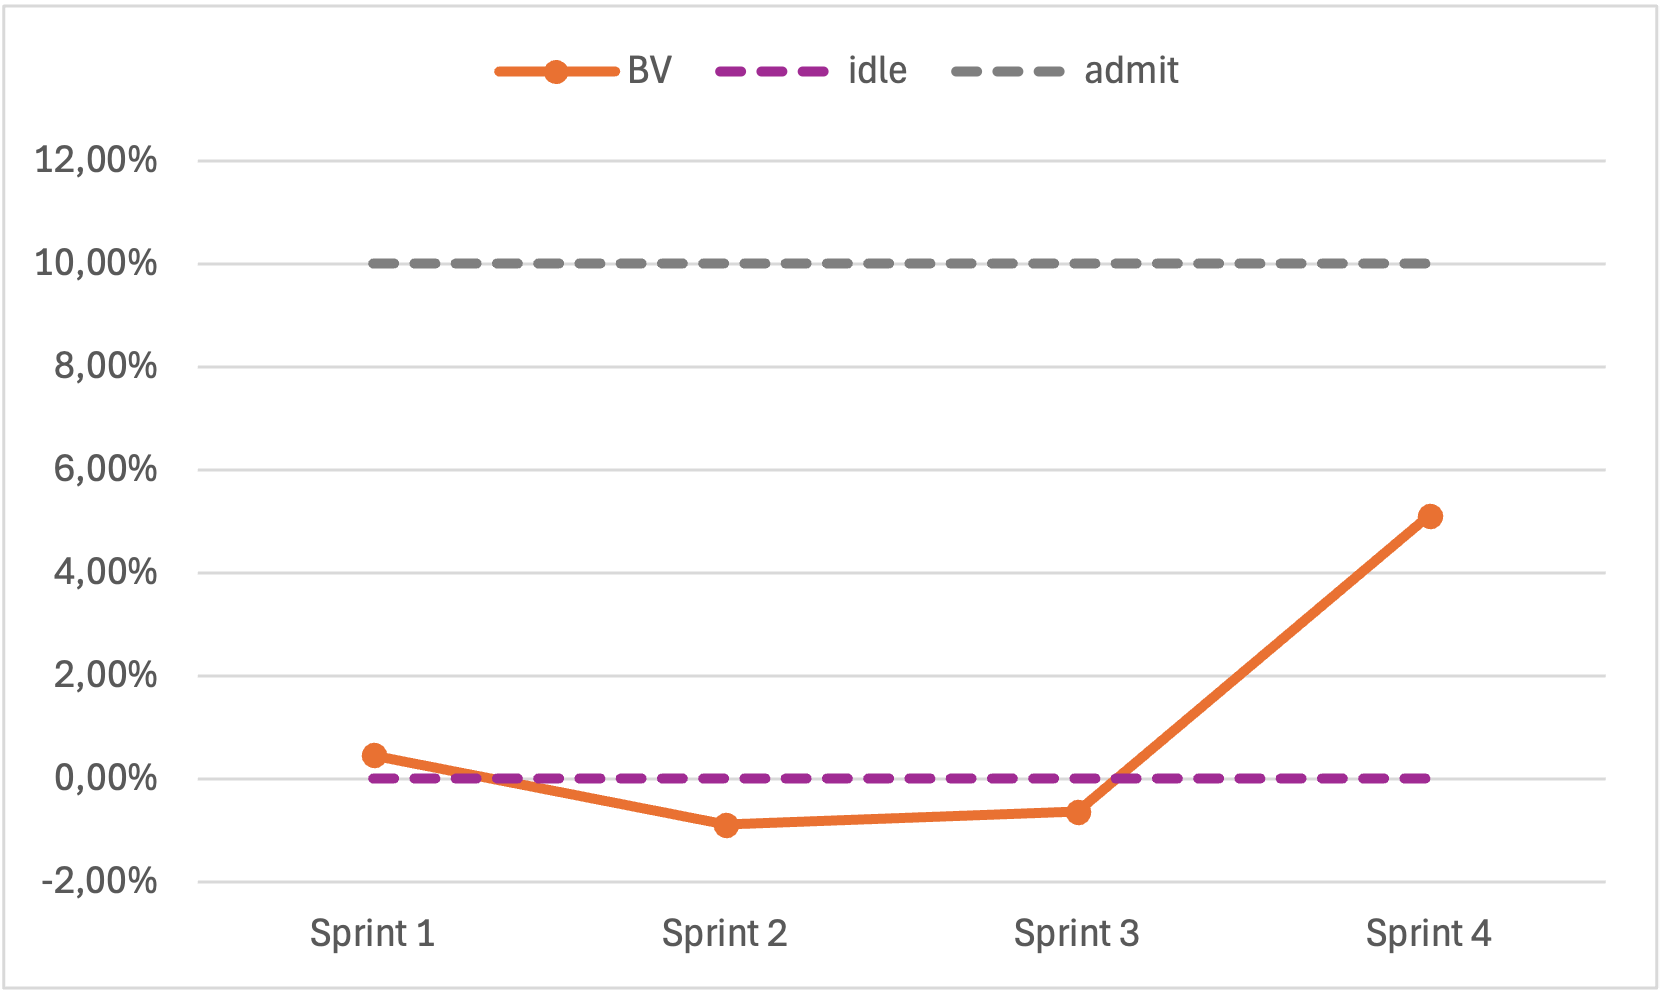
\includegraphics[width=0.8\textwidth]{./images/BV.png}
    \caption{Estimated To Compliation, Estimated At Compliation}
\end{figure}
\subsubsubsection*{Analisi}
Anche se la Budget Variance è sempre rimasta nei limiti ammissibili, è evidente come nel quarto sprint, dove la variazione è notevole, le ore preventivate fossero insufficienti e questo deve spingere a una più corretta pianificazione basata sulle retrospettive precedenti.

\subsubsection{Cost Variance, Schedule Variance}
\begin{figure}[H]
    \centering
    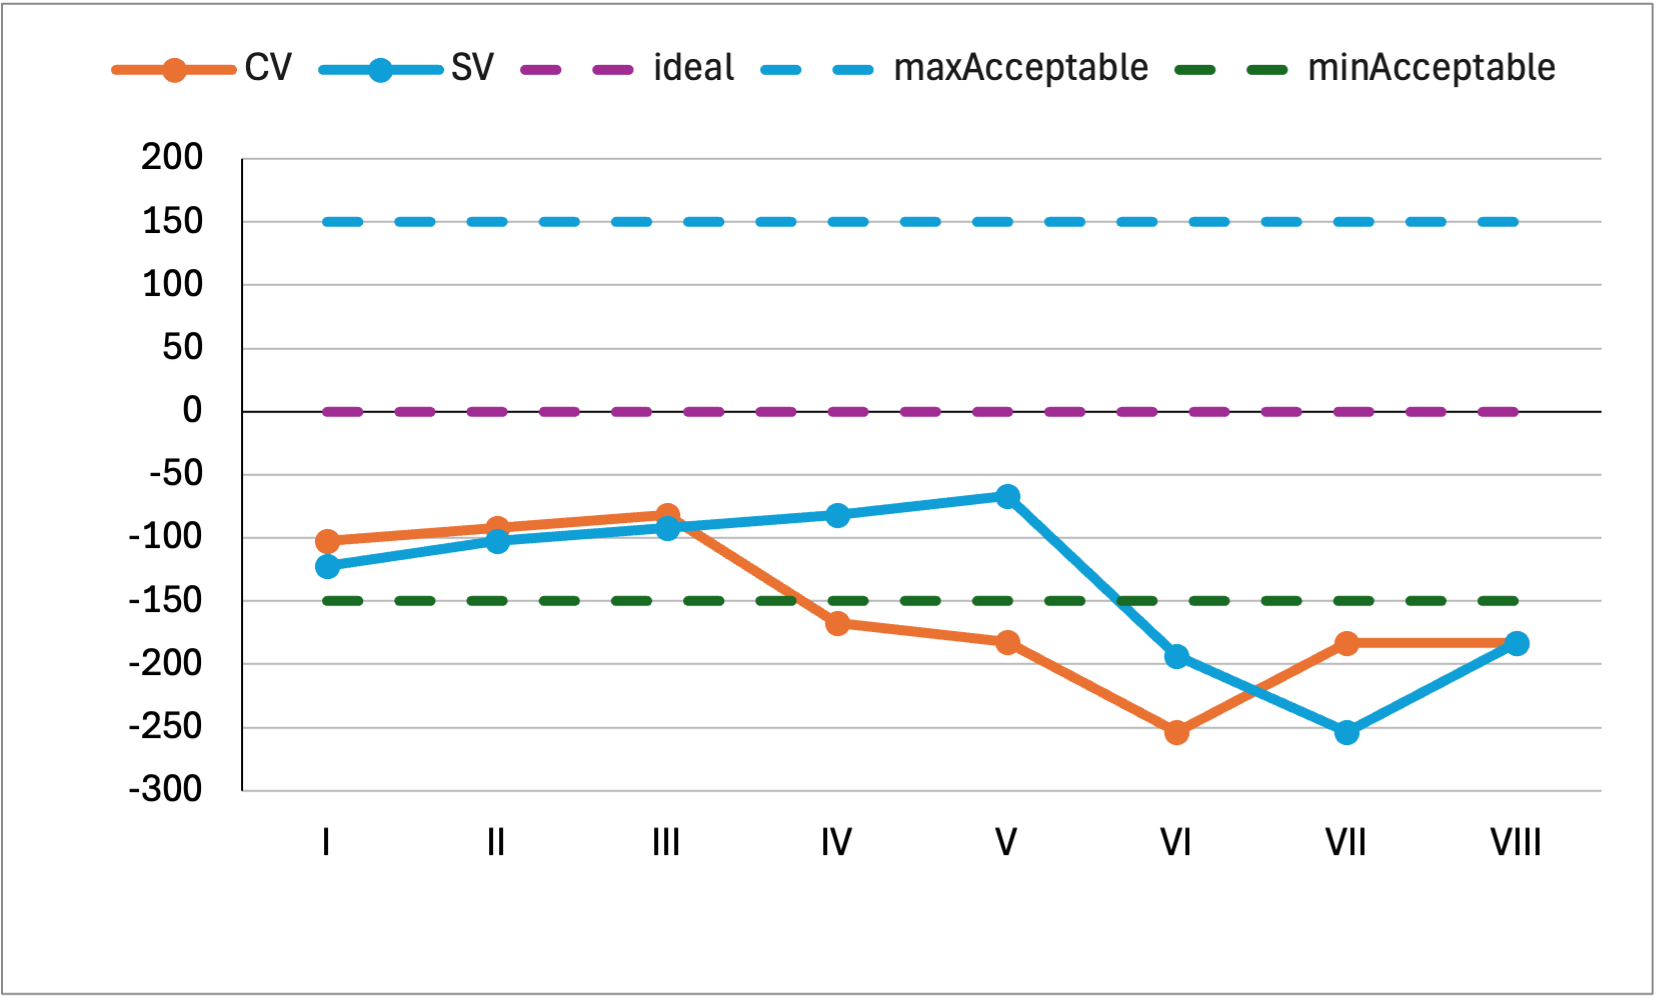
\includegraphics[width=0.8\textwidth]{./images/CV-SV.png}
    \caption{Cost Variance, Schedule Variance}
\end{figure}
\subsubsubsection*{Analisi}
Per quanto i valori, soprattutto della Schedule Variance, siano praticamente sempre rimasti accettabili, non si notano dei netti miglioramenti, ma anzi un peggioramento, come in altre metriche, nel corso del quarto sprint. Questo deve spingere a una migliore gestione delle risorse per il raggiungimento degli obiettivi entro i costi preventivati.

\subsubsection{Cost Performace Index}
\begin{figure}[H]
    \centering
    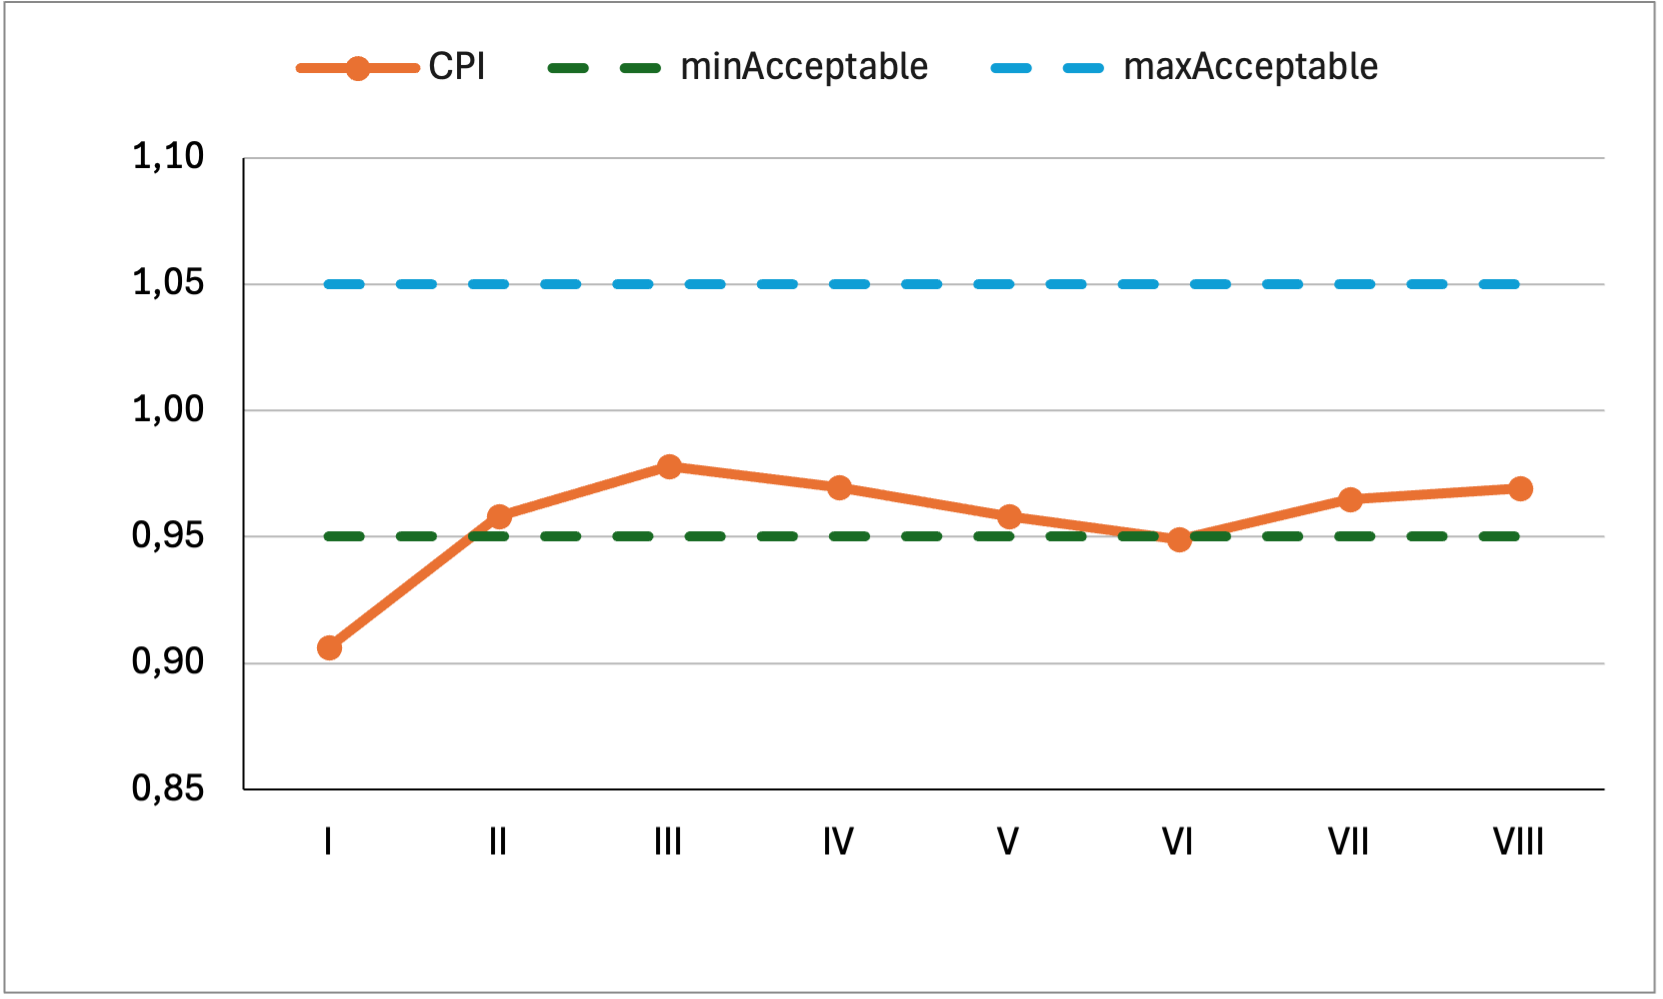
\includegraphics[width=0.8\textwidth]{./images/CPI.png}
    \caption{Cost Performace Index}
\end{figure}
\subsubsubsection*{Analisi}
È evidente come il Cost Performace Index sia migliorato nel corso degli sprint, fino a rientrare nei limiti ammissibli, l'obiettivo deve essere quello di seguire il trend attuale per puntare al valore ideale.

\subsection{Qualità di processo - Documentazione}
\subsubsection{Indice di Gulpease}
\begin{figure}[H]
    \centering
    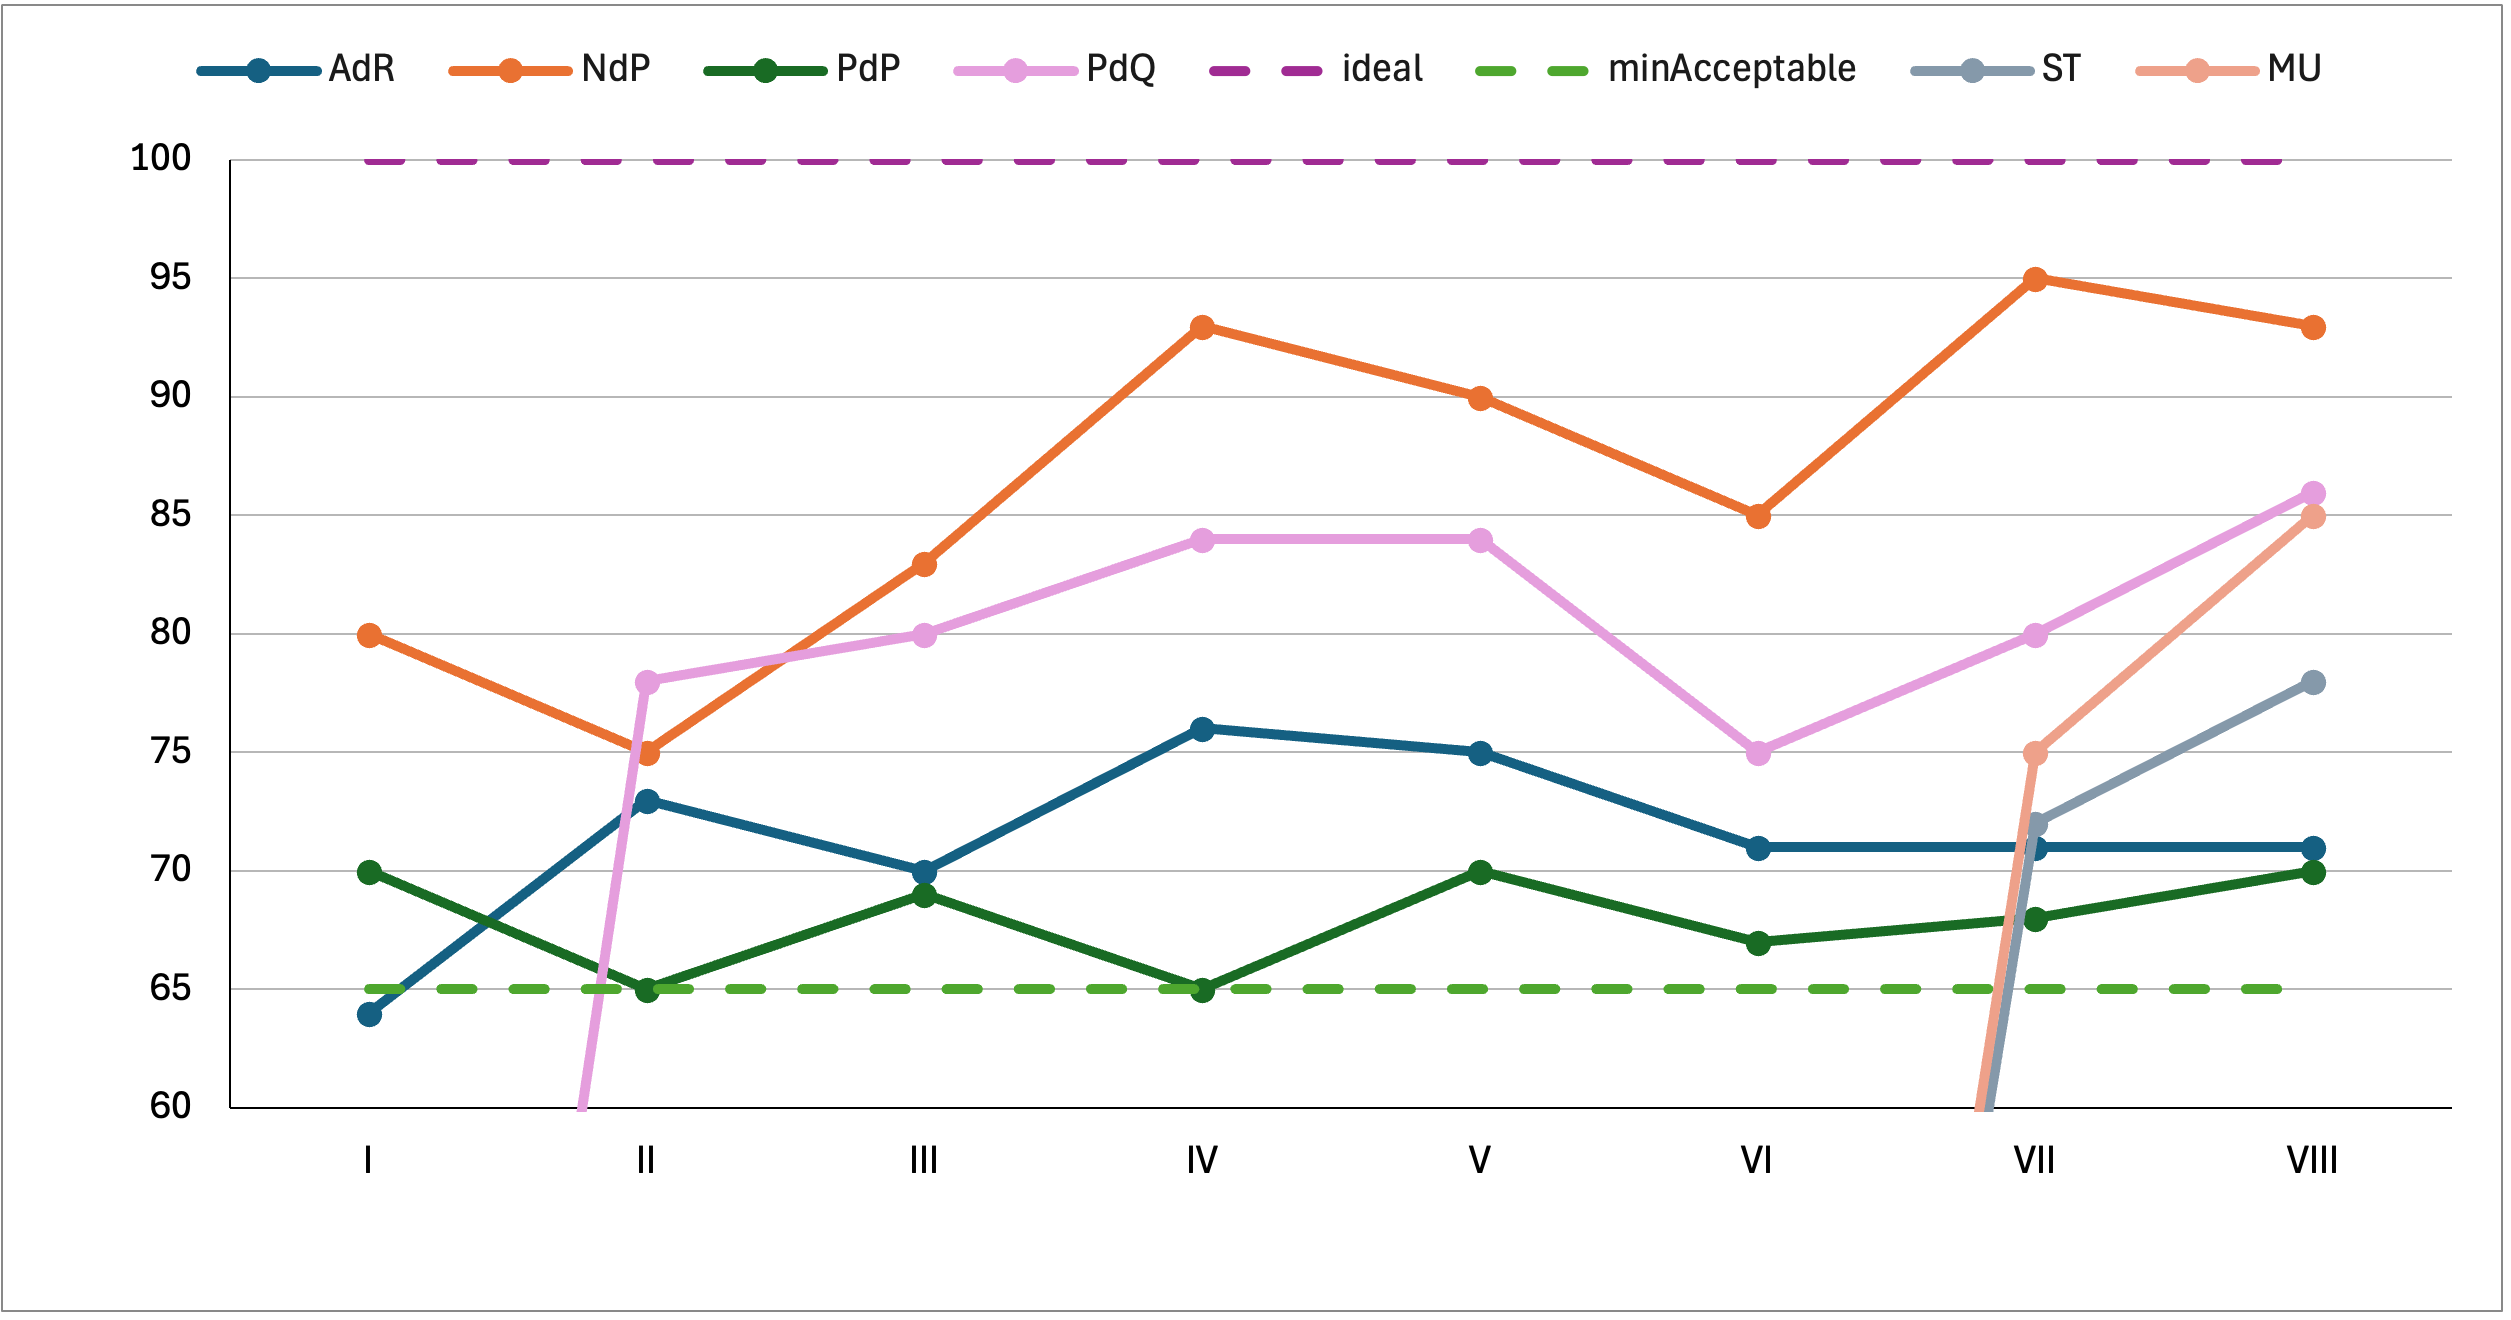
\includegraphics[width=0.8\textwidth]{./images/gulpease.png}
    \caption{Indice di Gulpease}
\end{figure}
\subsubsubsection*{Analisi}
Al termine del secondo sprint tutti i documenti erano in lavorazione ed entro i limiti minimi di leggibilità, si nota peraltro un miglioramento nella leggibilità di tutti i documenti ad esclusione del Piano di Progetto, sul quale il gruppo dovrà concentrarsi di più per garantire una scrittura comprensibile.


\subsection{Qualità di processo - Gestione della qualità}
\subsubsection{Metriche non soddisfatte}
\begin{figure}[H]
    \centering
    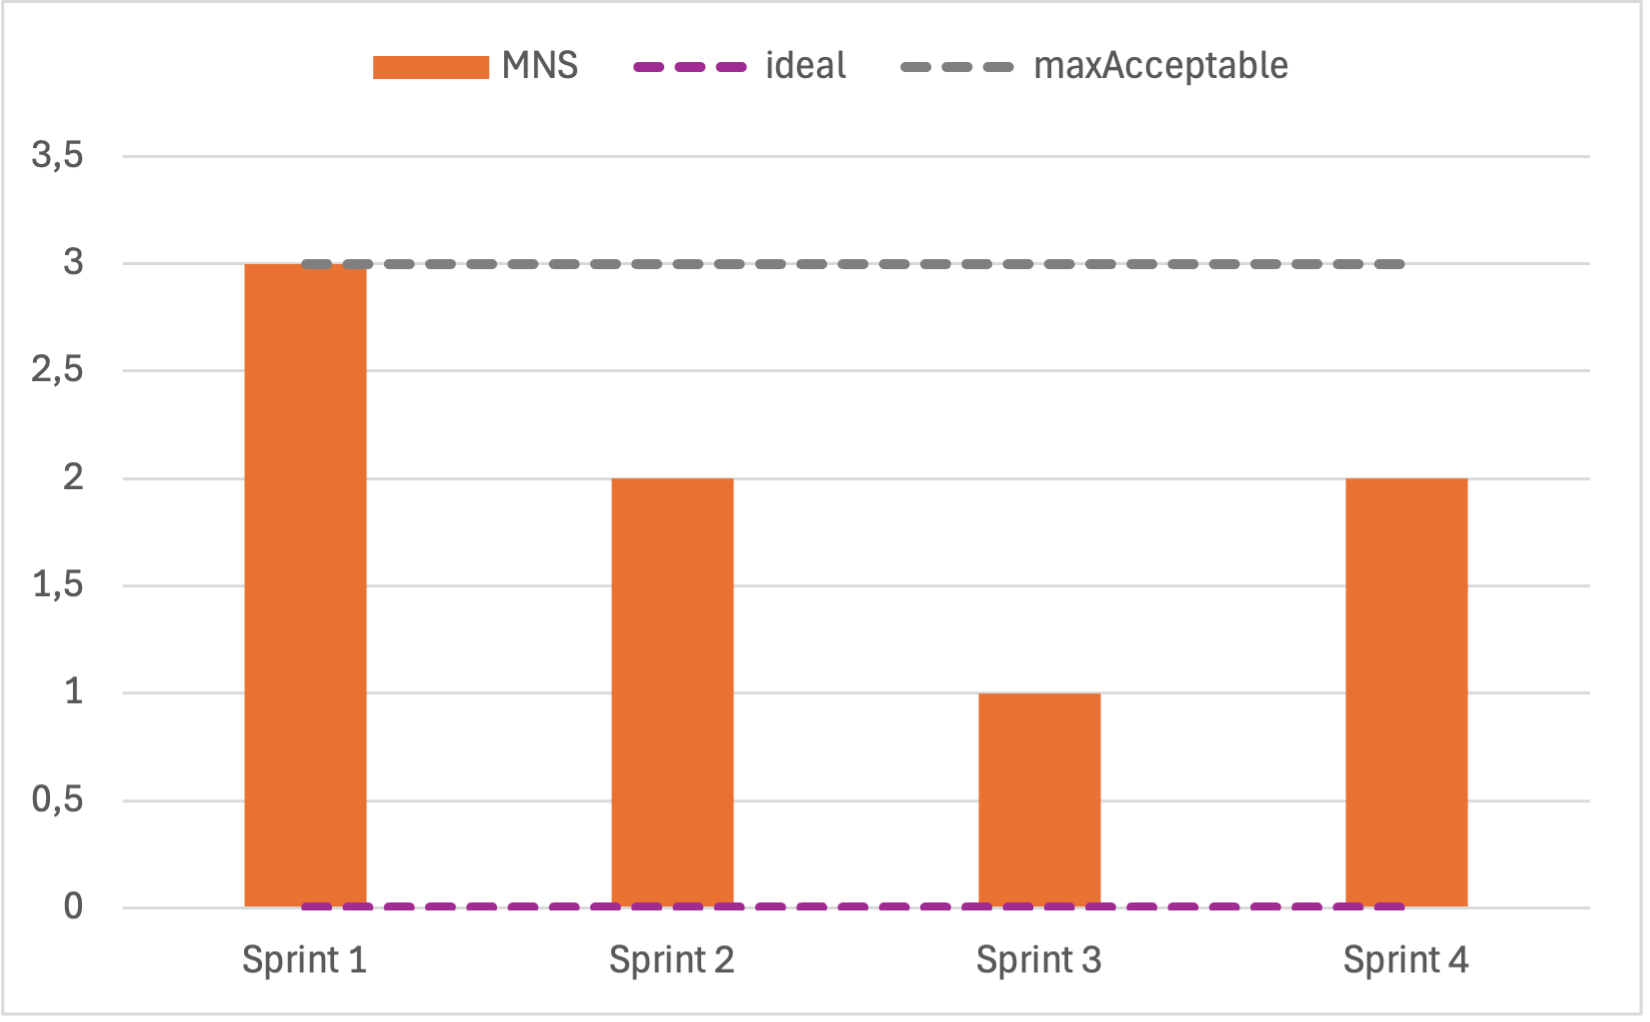
\includegraphics[width=0.8\textwidth]{./images/MNS.png}
    \caption{Metriche non soddisfatte}
\end{figure}
\subsubsubsection*{Analisi}
La metrica che non risulta mai soddisfatta è EAC per la quale si rimanda all'analisi specifica. Altre metriche che risultano non sddisfatte sono ETC (primi due sprint), CPI (primo sprint) e CV (quarto sprint per il quale si rimanda all'analisi specifica).



\subsection{Qualità di prodotto - Funzionalità}
\subsubsection{Requisiti soddisfatti}
\begin{figure}[H]
    \centering
    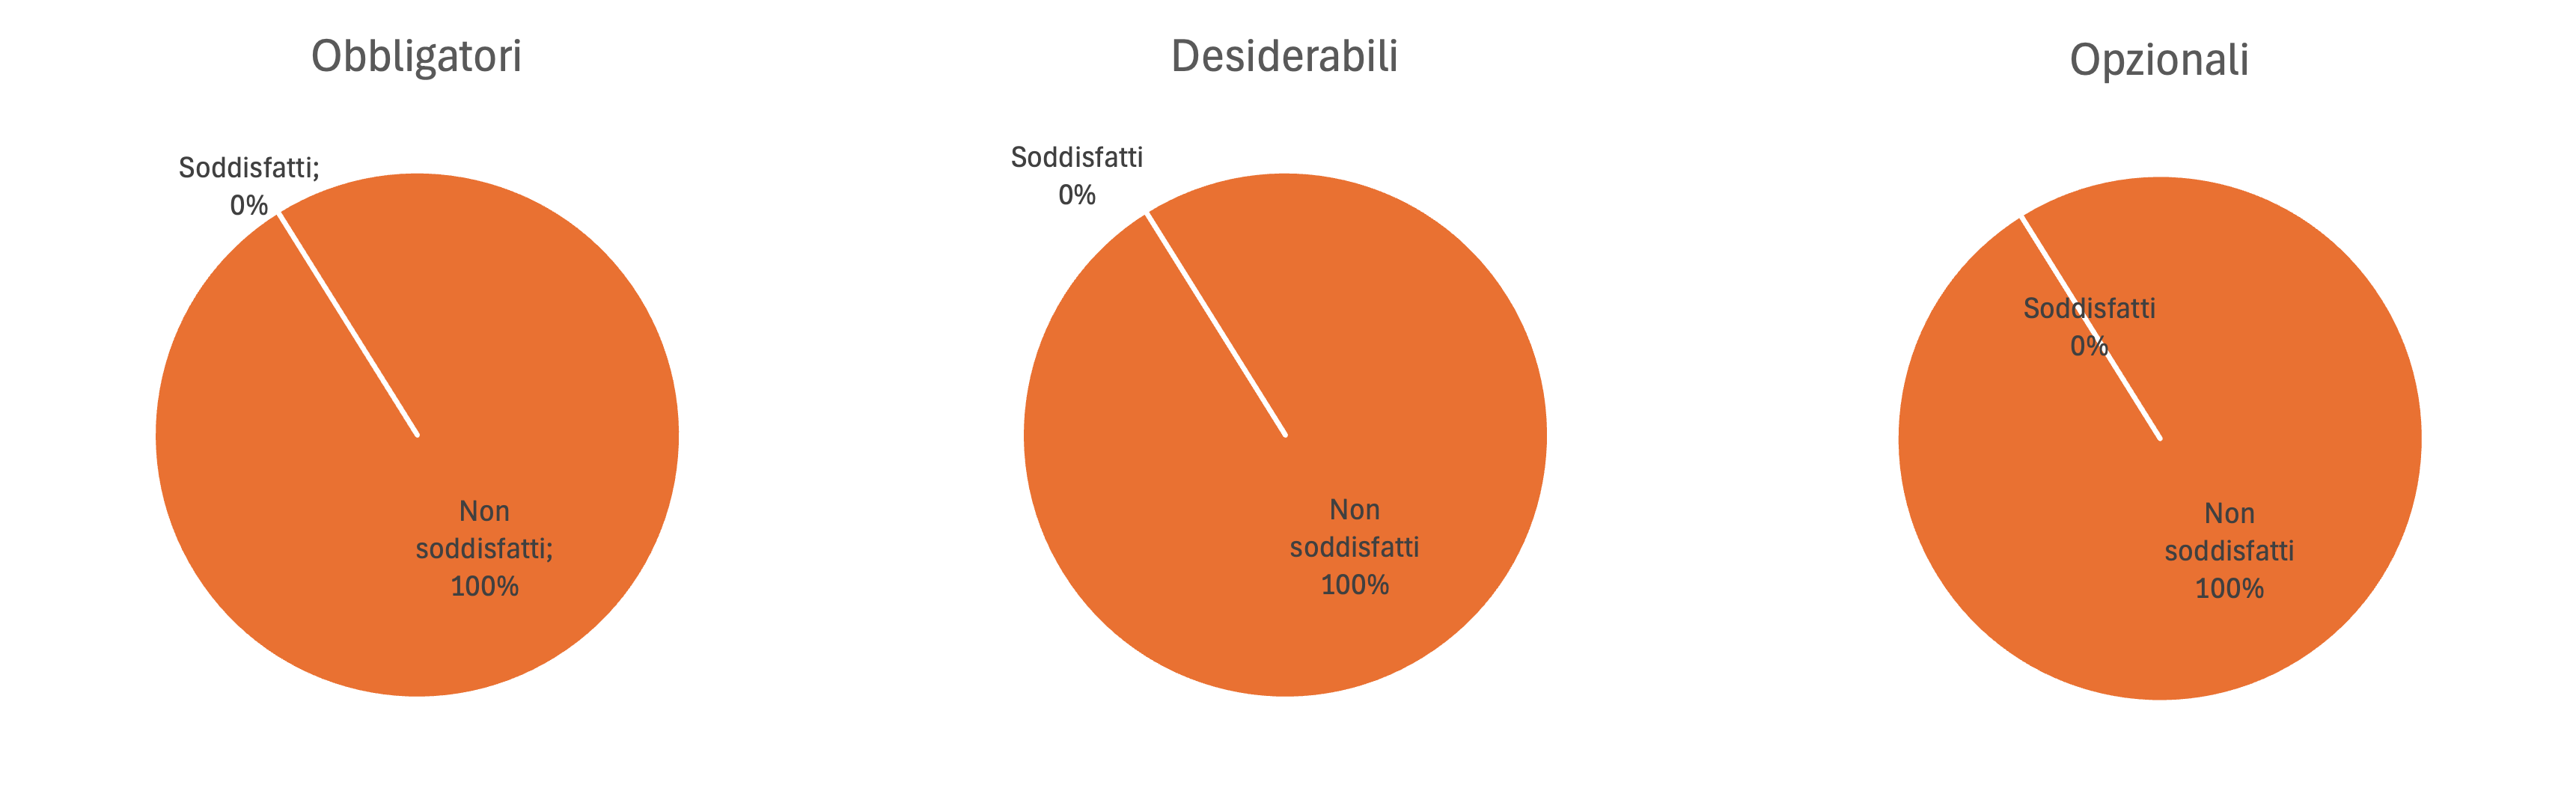
\includegraphics[width=0.8\textwidth]{./images/requisitisoddisfatti.png}
    \caption{Requisiti soddisfatti}
\end{figure}
\subsubsubsection*{Analisi}
Il progetto fino ad ora si è concentrato sulla creazione di un \textit{Proof of Concept}\textsubscript{G}, e non su prodotto finale con il quale soddisfare i requisiti, per cui è normale che nel cruscotto non risulti soddisfatto alcun requisito.



\subsection{Considerazioni finali in vista della revisione RTB}
Sin dalle prime fasi del progetto il gruppo si è posto l'obiettivo di avere un \textit{Way of Working}\textsubscript{G} chiaro e puntuale, anche se di natura incrementale, in quanto questo deve essere gradualmente ampliato e raffinato con il passare del tempo. Nonostante il \textit{Way of Working}\textsubscript{G}  sia progressivamente migliorato con l’avanzare del progetto, alcune aree necessitano di essere ancora migliorate per far si che la qualità di processo si rifletta positivamente sulla qualità di prodotto. \\
La comunicazione, all'interno del team e con il Proponente\textsubscript{G} è stata fin da subito stabile e costruttiva, sia in modalità sincrona, permettendo riunioni efficaci di durata non eccessiva, che asincrona, permettendo una buona organizzazione del lavoro. \\
Il processo di automiglioramento che il gruppo si è impegnato ad assumere si è concentrato, e continuerà a concentrarsi, anche sulle modalità di gestione delle difficoltà e degli imprevisti, per escogitare contromisure efficaci che permettano di non sprecare risorse\textsubscript{G}. \\
Un obiettivo di vitale importanza per il gruppo nel corso dei prossimi sprint è l'aggiornamento rigoroso e puntuale del Piano di Progetto e del Piano di Qualifica con i dati rilevanti ed aggionati, al fine da poter essere sfruttati al meglio. \\



\end{document}
